% Apresentação — Projeto 11: Agrupando amostras sem usar os rótulos
% Compilar com XeLaTeX (usa a fonte Lato):  latexmk -xelatex apresentacao.tex
\documentclass[aspectratio=169,10pt,xcolor=table]{beamer}

\usepackage{fontspec}
\setsansfont{Lato}
\setmonofont{DejaVu Sans Mono}[Scale=0.82]
\newfontfamily\titlefont{Lato Black}
\usepackage{amsmath}
\usepackage{booktabs}
\usepackage{tikz}
\usetikzlibrary{arrows.meta,positioning,calc,shapes.misc,shadows}
\usepackage{pgfplots}
\pgfplotsset{compat=1.18}
\pgfkeys{/pgf/number format/.cd,assume math mode=true,use comma,1000 sep={.}}
\pgfplotsset{numfont/.style={xticklabel={\pgfmathprintnumber{\tick}},yticklabel={\pgfmathprintnumber{\tick}}}}
\usepackage[most]{tcolorbox}
\usepackage{listings}

\graphicspath{{../results/}}

% ------------------------------------------------------------------ Cores
\definecolor{navy}{HTML}{12409A}
\definecolor{dark}{HTML}{0A2A5E}
\definecolor{titlecol}{HTML}{0D2F6E}
\definecolor{bg}{HTML}{F2F3F5}
\definecolor{ink}{HTML}{1E2433}
\definecolor{muted}{HTML}{5B6272}
\definecolor{rule}{HTML}{D9DCE3}
\definecolor{accent}{HTML}{EB6834}
\definecolor{okc}{HTML}{1BAF7A}
\definecolor{errc}{HTML}{E34948}
\definecolor{c1}{HTML}{2A78D6}
\definecolor{c2}{HTML}{EB6834}
\definecolor{c3}{HTML}{1BAF7A}
\definecolor{c4}{HTML}{EDA100}
\definecolor{c5}{HTML}{E87BA4}

% ------------------------------------------------------------------ Tema
\setbeamertemplate{navigation symbols}{}
\setbeamercolor{normal text}{fg=ink}
\setbeamercolor{structure}{fg=navy}
\setbeamercolor{alerted text}{fg=accent}
\setbeamerfont{normal text}{size=\small}
\setbeamersize{text margin left=0.9cm,text margin right=0.9cm}

\setbeamertemplate{itemize item}{\raisebox{0.15ex}{\tikz\fill[navy] (0,0) circle (0.42ex);}}
\setbeamertemplate{itemize subitem}{\raisebox{0.15ex}{\tikz\draw[navy,line width=0.5pt] (0,0) circle (0.38ex);}}
\setlength{\leftmargini}{1.1em}

% Rótulo da parte (quem apresenta), mostrado no rodapé
\newcommand{\partlabel}{}
\newcommand{\setpart}[1]{\renewcommand{\partlabel}{#1}}

% Fundo das páginas de conteúdo: cantos decorativos inspirados no esboço
\newcommand{\hatch}[1]{% hachura branca dentro da região já recortada
  \foreach \i in {-3,-2.85,...,3}{\draw[white,line width=0.9pt] (#1) ++(\i,-1.5) -- ++(3,3);}}
\setbeamertemplate{background canvas}{%
  
\begin{tikzpicture}
    \useasboundingbox (0,0) rectangle (\paperwidth,\paperheight);
    \fill[bg] (0,0) rectangle (\paperwidth,\paperheight);
    % canto superior esquerdo
    \fill[navy] (0,9) -- (2.2,9) -- (0,8.0) -- cycle;
    \begin{scope}\clip (0,9) -- (2.2,9) -- (0,8.0) -- cycle;
      \fill[dark] (1.35,8.35) circle (0.42); \end{scope}
    \begin{scope}\clip (0,9) -- (0.85,9) -- (0,8.6) -- cycle;
      \fill[navy] (0,8.5) rectangle (1,9); \hatch{0.4,8.8} \end{scope}
    % canto inferior direito
    \fill[navy] (16,0) -- (13.6,0) -- (16,1.05) -- cycle;
    \begin{scope}\clip (16,0) -- (13.6,0) -- (16,1.05) -- cycle;
      \fill[dark] (14.75,0.62) circle (0.45); \end{scope}
  \end{tikzpicture}}

\setbeamertemplate{frametitle}{%
  \vspace*{0.30cm}\centering
  {\titlefont\fontsize{15}{17}\selectfont\color{titlecol}\MakeUppercase{\insertframetitle}\par}
  \ifx\insertframesubtitle\empty\else
    \vspace{1pt}{\footnotesize\color{muted}\insertframesubtitle\par}\fi
  \vspace{-0.05cm}}

\setbeamertemplate{footline}{%
  \begin{tikzpicture}
    \useasboundingbox (0,0) rectangle (16,0.55);
    \node[text=white,font=\scriptsize\bfseries] at (15.55,0.26) {\insertframenumber};
  \end{tikzpicture}}

% ------------------------------------------------------------------ Caixas
\tcbset{
  base/.style={enhanced,colback=white,colframe=white,boxrule=0pt,arc=1.6mm,
    left=2.2mm,right=2.2mm,top=1.6mm,bottom=1.6mm,fontupper=\small,before upper=\raggedright,
    drop fuzzy shadow={black!8}},
}
\newtcolorbox{card}[2][]{base,title={#2},coltitle=white,colbacktitle=navy,
  fonttitle=\bfseries\small,toptitle=0.6mm,bottomtitle=0.6mm,#1}
\newtcolorbox{plain}[1][]{base,#1}
\newtcolorbox{banner}[1][]{enhanced,colback=navy,colframe=navy,arc=1.6mm,boxrule=0pt,
  coltext=white,halign=center,valign=center,fontupper=\bfseries,
  left=3mm,right=3mm,top=2mm,bottom=2mm,#1}
\newtcolorbox{callout}[1][]{enhanced,colback=accent!10,colframe=accent,boxrule=0pt,
  leftrule=1.2mm,arc=0.6mm,left=2mm,right=2mm,top=1.2mm,bottom=1.2mm,fontupper=\footnotesize,#1}

\newcommand{\bignum}[2]{{\titlefont\fontsize{20}{22}\selectfont\color{#1}#2}}
% "chip" com a chamada principal do código
\newcommand{\code}[1]{\tikz[baseline=(c.base)]\node[fill=white,draw=rule,rounded corners=1mm,inner sep=2.5pt,font=\ttfamily\scriptsize,text=navy] (c) {#1};}
\newcommand{\nbsec}[1]{{\color{muted}\scriptsize notebook §#1}}

% ------------------------------------------------------------------ Código
\lstdefinestyle{py}{
  language=Python,basicstyle=\ttfamily\scriptsize\color{ink},
  keywordstyle=\color{navy}\bfseries,commentstyle=\color{muted}\itshape,
  stringstyle=\color{accent!85!black},showstringspaces=false,
  columns=fullflexible,keepspaces=true,breaklines=true,
  backgroundcolor=\color{white},frame=leftline,framerule=1.2pt,rulecolor=\color{navy},
  xleftmargin=6pt,framexleftmargin=4pt,aboveskip=2pt,belowskip=2pt,
  extendedchars=true,inputencoding=utf8,
  literate={á}{{\'a}}1 {ã}{{\~a}}1 {â}{{\^a}}1 {à}{{\`a}}1 {é}{{\'e}}1 {ê}{{\^e}}1
           {í}{{\'i}}1 {ó}{{\'o}}1 {õ}{{\~o}}1 {ô}{{\^o}}1 {ú}{{\'u}}1 {ç}{{\c c}}1
           {→}{{$\rightarrow$}}1 {≈}{{$\approx$}}1,
  morekeywords={True,False,None},
}
\lstset{style=py}

% ================================================================== DOCUMENTO
\begin{document}

% ================================================================== PARTE 1
\setpart{Parte 1 · Leonardo Demore}

% ------------------------------------------------------------------ 1. Capa
{
\setbeamertemplate{background canvas}{%
  
\begin{tikzpicture}
    \useasboundingbox (0,0) rectangle (\paperwidth,\paperheight);
    \fill[bg] (0,0) rectangle (\paperwidth,\paperheight);
    \fill[navy] (0,9) -- (5.2,9) -- (0,6.6) -- cycle;
    \begin{scope}\clip (0,9) -- (5.2,9) -- (0,6.6) -- cycle;
      \fill[dark] (3.1,7.75) circle (1.0); \end{scope}
    \begin{scope}\clip (0,9) -- (2.0,9) -- (0,8.05) -- cycle;
      \fill[navy] (0,8) rectangle (2,9); \hatch{1,8.5} \end{scope}
    \fill[navy] (16,0) -- (10.8,0) -- (16,2.4) -- cycle;
    \begin{scope}\clip (16,0) -- (10.8,0) -- (16,2.4) -- cycle;
      \fill[dark] (12.9,1.25) circle (1.0); \end{scope}
    \begin{scope}\clip (16,0) -- (14,0) -- (16,0.95) -- cycle;
      \fill[navy] (14,0) rectangle (16,1); \hatch{15,0.5} \end{scope}
  \end{tikzpicture}}
\begin{frame}[plain]
  \centering
  \vspace*{0.8cm}
  {\titlefont\fontsize{27}{31}\selectfont\color{titlecol}
   AGRUPAMENTO NÃO\\SUPERVISIONADO EM\\EXPRESSÃO GÊNICA\par}
  \vspace{0.3cm}
  {\normalsize\color{muted}Projeto 11 — Agrupando amostras sem usar os rótulos\par}
  \vspace{0.45cm}
  {\small
  \begin{tabular}{rl}
    \textbf{Leonardo Demore} {\color{muted}(15674786)} & {\color{muted}· problema e dados}\\
    \textbf{Thiago Tavares} {\color{muted}(15490194)} & {\color{muted}· métodos de agrupamento}\\
    \textbf{Julio Fuganti} {\color{muted}(15638792)} & {\color{muted}· validação e conclusões}
  \end{tabular}\par}
  \vspace{0.3cm}
  {\footnotesize\color{muted}SCC02713 · Introdução à Bioinformática · ICMC/USP\par}
\end{frame}
}

% ------------------------------------------------------------------ 2. Pergunta
\begin{frame}{O problema}
  \vspace{0.35cm}
  \begin{columns}[T,onlytextwidth]
    \column{0.315\textwidth}
    \begin{card}[height=2.7cm,fontupper=\normalsize]{1 · Rótulos escondidos}
      \begin{itemize}
        \item Tipo de tumor \textbf{guardado}
        \item Usado só no fim, para \textbf{conferir}
      \end{itemize}
    \end{card}
    \column{0.315\textwidth}
    \begin{card}[height=2.7cm,fontupper=\normalsize]{2 · Agrupar pela expressão}
      \begin{itemize}
        \item Amostras \textbf{parecidas} no mesmo grupo
        \item Semelhança = \textbf{distância} entre perfis
      \end{itemize}
    \end{card}
    \column{0.315\textwidth}
    \begin{card}[height=2.7cm,fontupper=\normalsize,colbacktitle=accent]{3 · Não supervisionado}
      \begin{itemize}
        \item Sem \textbf{resposta certa} no ajuste
        \item O método só vê os \textbf{dados}
      \end{itemize}
    \end{card}
  \end{columns}
  \vspace{0.45cm}
  \begin{banner}
    \Large A expressão gênica, sozinha,\\ redescobre os 5 tipos de tumor?
  \end{banner}
\end{frame}

% ------------------------------------------------------------------ 3. Dados
\begin{frame}{Os dados}
  \framesubtitle{Gene expression cancer RNA-Seq — UCI / TCGA Pan-Cancer}
  \vspace{0.25cm}
  \begin{columns}[T,onlytextwidth]
    \column{0.44\textwidth}
    \begin{plain}
      \centering
      \begin{tabular}{ccc}
        \bignum{navy}{801} & \bignum{muted}{×} & \bignum{navy}{20.531}\\
        {\footnotesize amostras} & & {\footnotesize genes}
      \end{tabular}
    \end{plain}
    \vspace{0.2cm}
    \begin{itemize}\normalsize\setlength{\itemsep}{4pt}
      \item Cada amostra é um \textbf{ponto em 20.531 dimensões}
      \item 5 tipos de tumor, \textbf{desbalanceados}
      \item Rótulos guardados até a etapa 4
    \end{itemize}
    \column{0.52\textwidth}
    \begin{plain}
      {\footnotesize\bfseries Amostras por tipo de tumor}\par
      \centering
      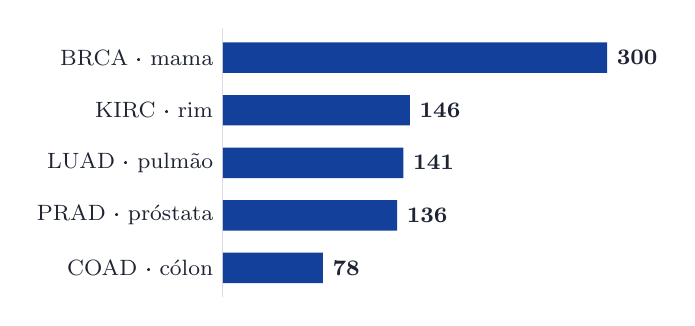
\begin{tikzpicture}
        \begin{axis}[xbar, width=7.6cm, height=5.0cm, bar width=11pt,
            xmin=0, xmax=370, axis x line=none, axis y line*=left,
            ytick={1,...,5}, y axis line style={draw=rule},
            yticklabels={{COAD · cólon},{PRAD · próstata},{LUAD · pulmão},{KIRC · rim},{BRCA · mama}},
            yticklabel style={font=\footnotesize,text=ink}, major tick length=0pt,
            nodes near coords={\pgfmathprintnumber{\pgfplotspointmeta}},
            nodes near coords style={font=\footnotesize\bfseries,text=ink},
            enlarge y limits=0.14]
          \addplot[fill=navy,draw=none] coordinates {(78,1) (136,2) (141,3) (146,4) (300,5)};
        \end{axis}
      \end{tikzpicture}
    \end{plain}
  \end{columns}
\end{frame}

% ------------------------------------------------------------------ 4. Pipeline
\begin{frame}{Pipeline}
  \framesubtitle{Etapas do processamento}
  \vspace{0.6cm}
  \centering
  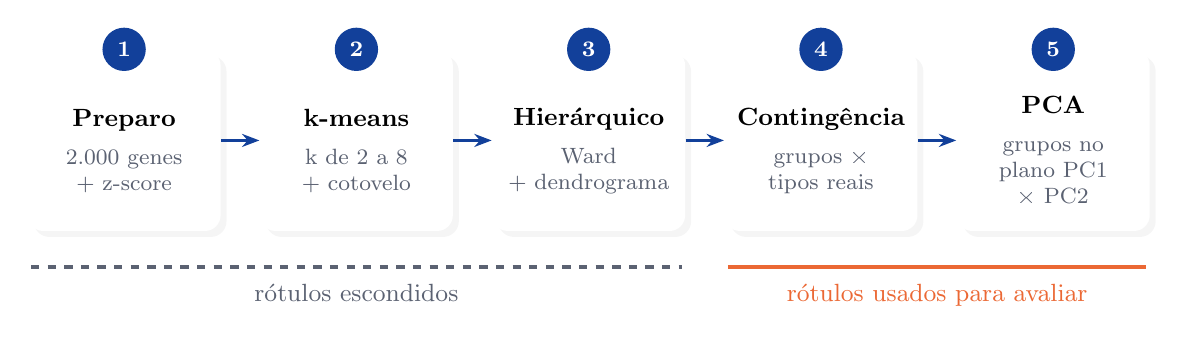
\begin{tikzpicture}[
      stepbox/.style={draw=none,fill=white,rounded corners=2mm,minimum width=2.45cm,
        minimum height=2.3cm,text width=2.3cm,align=center,font=\footnotesize,inner sep=2pt,
        drop shadow={opacity=0.08}},
      num/.style={circle,fill=navy,text=white,font=\footnotesize\bfseries,minimum size=0.55cm,inner sep=0},
      arr/.style={-{Stealth[length=2.2mm]},line width=1.2pt,color=navy}]
    \foreach \x/\n/\t/\d in {
        0/1/Preparo/2.000 genes\\+ z-score,
        2.95/2/k-means/k de 2 a 8\\+ cotovelo,
        5.9/3/Hierárquico/Ward\\+ dendrograma,
        8.85/4/Contingência/grupos ×\\tipos reais,
        11.8/5/PCA/grupos no\\plano PC1 × PC2}{
      \node[stepbox] (s\n) at (\x,0) {\rule{0pt}{14pt}{\small\textbf{\t}}\\[4pt]{\color{muted}\d}};
      \node[num] at (s\n.north) {\n};
    }
    \foreach \a/\b in {1/2,2/3,3/4,4/5} \draw[arr] (s\a.east) -- (s\b.west);
    \draw[line width=1.6pt,muted,dashed] ($(s1.south west)+(0.05,-0.45)$) -- ($(s3.south east)+(-0.05,-0.45)$)
      node[midway,below=2pt,font=\small,text=muted] {rótulos escondidos};
    \draw[line width=1.6pt,accent] ($(s4.south west)+(0.05,-0.45)$) -- ($(s5.south east)+(-0.05,-0.45)$)
      node[midway,below=2pt,font=\small,text=accent] {rótulos usados para avaliar};
  \end{tikzpicture}
  \vspace{0.6cm}

  {\footnotesize\color{muted}\textbf{Pacotes usados:}\par
  pandas · scikit-learn · SciPy · matplotlib — semente fixa (42) para reprodutibilidade\par}
\end{frame}

% ------------------------------------------------------------------ 5. Pré-processamento
\begin{frame}{Pré-processamento}
  \framesubtitle{\nbsec{1.4–1.6}}
  \vspace{0.2cm}
  \begin{columns}[T,onlytextwidth]
    \column{0.48\textwidth}
    \begin{card}[height=5.6cm]{1 · Filtrar: 2.000 genes mais variáveis}
      \centering
      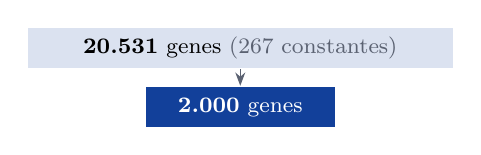
\begin{tikzpicture}[font=\footnotesize]
        \fill[navy!15] (0,0) rectangle (5.4,0.5);
        \node at (2.7,0.25) {\textbf{20.531} genes \color{muted}(267 constantes)};
        \fill[navy] (1.5,-0.75) rectangle (3.9,-0.25);
        \node[text=white] at (2.7,-0.5) {\textbf{2.000} genes};
        \draw[-{Stealth},muted] (2.7,-0.02) -- (2.7,-0.23);
      \end{tikzpicture}\par\vspace{4pt}
      \raggedright
      \begin{itemize}\setlength{\itemsep}{2pt}
        \item Genes quase constantes = \textbf{ruído} na distância
        \item Variância medida \textbf{antes} do z-score
        \item Não usa os rótulos
      \end{itemize}
      \vfill\code{expression.var(axis=0)}
    \end{card}
    \column{0.48\textwidth}
    \begin{card}[height=5.6cm]{2 · Padronizar: z-score por gene}
      \centering
      $\displaystyle z_{ig}=\frac{x_{ig}-\bar{x}_g}{s_g}$\par\vspace{6pt}
      \raggedright
      \begin{itemize}\setlength{\itemsep}{2pt}
        \item Os métodos usam \textbf{distância euclidiana}
        \item Sem padronizar, um gene pesaria até \textbf{10× mais} que outro
        \item Resultado: matriz \textbf{801 × 2.000}
      \end{itemize}
      \vfill\code{StandardScaler().fit\_transform(...)}
    \end{card}
  \end{columns}
\end{frame}

% ================================================================== PARTE 2
\setpart{Parte 2 · Thiago Tavares}

% ------------------------------------------------------------------ 6. k-means
\begin{frame}{k-means}
  \framesubtitle{\nbsec{2.2}}
  \vspace{0.2cm}
  \begin{columns}[T,onlytextwidth]
    \column{0.44\textwidth}
    \begin{plain}
      \centering
      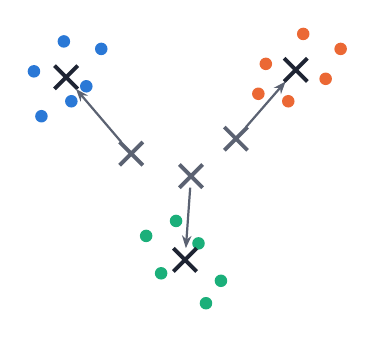
\begin{tikzpicture}[scale=0.95,
          pa/.style={circle,fill=c1,inner sep=1.6pt},
          pb/.style={circle,fill=c2,inner sep=1.6pt},
          pc/.style={circle,fill=c3,inner sep=1.6pt},
          cen/.style={cross out,draw=ink,line width=1.4pt,minimum size=7pt,inner sep=0}]
        \foreach \p in {(0.5,3.3),(0.9,3.7),(1.2,3.1),(0.6,2.7),(1.4,3.6),(1.0,2.9)} \node[pa] at \p {};
        \foreach \p in {(3.6,3.4),(4.1,3.8),(4.4,3.2),(3.9,2.9),(4.6,3.6),(3.5,3.0)} \node[pb] at \p {};
        \foreach \p in {(2.2,0.6),(2.7,1.0),(2.4,1.3),(3.0,0.5),(2.0,1.1),(2.8,0.2)} \node[pc] at \p {};
        \node[cen,draw=muted] (o1) at (1.8,2.2) {}; \node[cen] (n1) at (0.93,3.22) {};
        \node[cen,draw=muted] (o2) at (3.2,2.4) {}; \node[cen] (n2) at (4.0,3.32) {};
        \node[cen,draw=muted] (o3) at (2.6,1.9) {}; \node[cen] (n3) at (2.52,0.78) {};
        \foreach \i in {1,2,3} \draw[-{Stealth[length=1.6mm]},muted,thick] (o\i) -- (n\i);
      \end{tikzpicture}\par
      {\scriptsize\color{muted}os centros (×) caminham até a média do seu grupo}
    \end{plain}
    \column{0.52\textwidth}
    \begin{enumerate}\normalsize\setlength{\itemsep}{4pt}
      \item[\textbf{1.}] Sorteia $k$ centros
      \item[\textbf{2.}] Cada amostra vai para o \textbf{centro mais próximo}
      \item[\textbf{3.}] Centro vira a \textbf{média} do grupo
      \item[\textbf{4.}] Repete até estabilizar
    \end{enumerate}
    \vspace{2pt}
    \begin{card}{Minimiza a inércia}
      \centering
      $\displaystyle W(k)=\sum_{j=1}^{k}\sum_{i\in C_j}\lVert x_i-\mu_j\rVert^2$
    \end{card}
    \code{KMeans(n\_clusters=k, n\_init=10, random\_state=42)}\ {\scriptsize\color{muted}$k$ = 2 a 8}
  \end{columns}
\end{frame}

% ------------------------------------------------------------------ 7. Cotovelo
\begin{frame}{Método do cotovelo}
  \framesubtitle{\nbsec{2.4–2.5}}
  \vspace{0.1cm}
  \begin{columns}[T,onlytextwidth]
    \column{0.60\textwidth}
    \begin{plain}[left=1mm,right=1mm,top=1mm,bottom=1mm]
      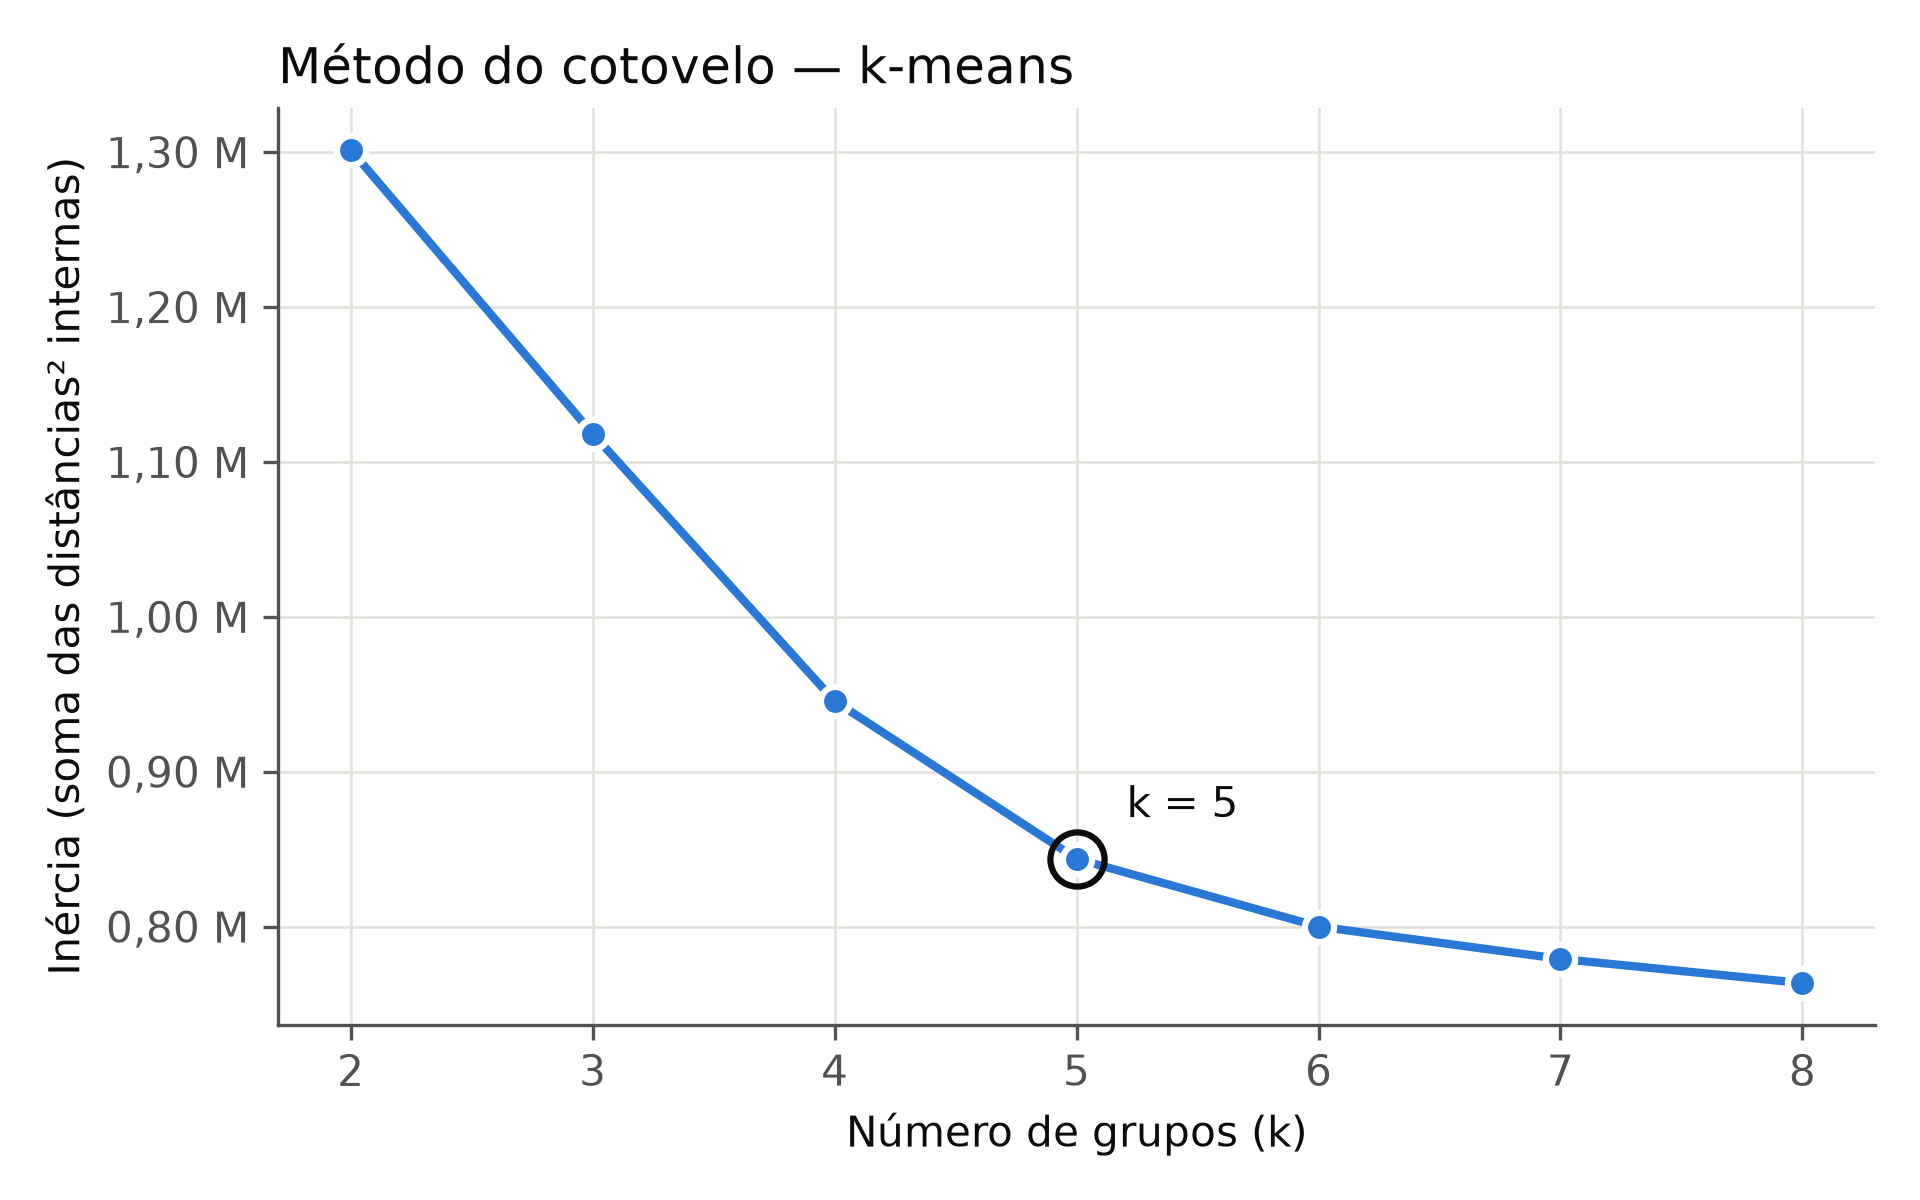
\includegraphics[width=\linewidth]{fig_cotovelo.png}
    \end{plain}
    \column{0.36\textwidth}
    \vspace{0.3cm}
    \begin{itemize}\normalsize\setlength{\itemsep}{6pt}
      \item A inércia \textbf{sempre cai} quando $k$ aumenta
      \item Buscamos onde a queda \textbf{deixa de compensar}
    \end{itemize}
    \vspace{0.2cm}
    \begin{plain}
      \centering\footnotesize
      \begin{tabular}{lc}
        Queda até $k=5$ & \textbf{10–15\%} por passo\\[2pt]
        Queda depois & \textbf{5\% ou menos}
      \end{tabular}
    \end{plain}
  \end{columns}
\end{frame}

% ------------------------------------------------------------------ 8. Critério automático
\begin{frame}{Escolhendo $k$ sem “olhômetro”}
  \framesubtitle{\nbsec{2.3}}
  \vspace{0.1cm}
  \begin{columns}[T,onlytextwidth]
    \column{0.46\textwidth}
    \begin{plain}[left=1mm,right=1mm]
      \centering
      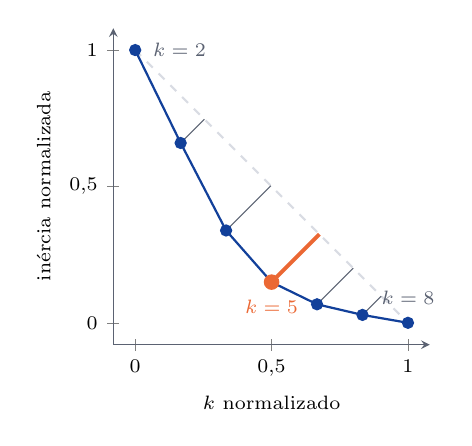
\begin{tikzpicture}
        \begin{axis}[width=6.8cm,height=5.6cm,axis equal image,
            xmin=-0.08,xmax=1.08,ymin=-0.08,ymax=1.08,
            xlabel={$k$ normalizado},ylabel={inércia normalizada},
            label style={font=\scriptsize},tick label style={font=\scriptsize},
            axis lines=left,axis line style={muted},xtick={0,0.5,1},ytick={0,0.5,1},
            numfont,clip=false]
          \addplot[rule,thick,dashed,domain=0:1] {1-x};
          \foreach \x/\y/\fx/\fy in {0.1667/0.6593/0.2537/0.7463, 0.3333/0.3385/0.4974/0.5026,
                                     0.6667/0.0679/0.7994/0.2006, 0.8333/0.0290/0.9022/0.0978}{
            \edef\tmp{\noexpand\draw[muted,thin] (axis cs:\x,\y) -- (axis cs:\fx,\fy);}\tmp}
          \draw[accent,line width=1.4pt] (axis cs:0.5,0.1492) -- (axis cs:0.6754,0.3246);
          \addplot[navy,thick,mark=*,mark size=1.8pt] coordinates
            {(0,1) (0.1667,0.6593) (0.3333,0.3385) (0.5,0.1492) (0.6667,0.0679) (0.8333,0.0290) (1,0)};
          \addplot[only marks,mark=*,mark size=2.6pt,accent] coordinates {(0.5,0.1492)};
          \node[font=\scriptsize,text=accent,anchor=north] at (axis cs:0.5,0.12) {$k=5$};
          \node[font=\scriptsize,text=muted,anchor=west] at (axis cs:0.03,1.0) {$k=2$};
          \node[font=\scriptsize,text=muted,anchor=south] at (axis cs:1,0.03) {$k=8$};
        \end{axis}
      \end{tikzpicture}
    \end{plain}
    \column{0.50\textwidth}
    \begin{itemize}\normalsize\setlength{\itemsep}{5pt}
      \item Eixos normalizados em $[0,1]$
      \item Cotovelo = ponto \textbf{mais distante} da reta entre os extremos
      \item Resultado: \textbf{$k = 5$}
    \end{itemize}
    \vspace{0.15cm}
    \begin{card}[colbacktitle=accent]{Mas foi por pouco}
      \centering
      \begin{tabular}{cc}
        \bignum{accent}{0,248} & \bignum{muted}{0,232}\\
        {\footnotesize distância de $k=5$} & {\footnotesize distância de $k=4$}
      \end{tabular}\par\vspace{3pt}
      {\footnotesize\raggedright O cotovelo é suave: é uma heurística, vale conferir com outro método.\par}
    \end{card}
  \end{columns}
\end{frame}

% ------------------------------------------------------------------ 9. Hierárquico
\begin{frame}{Agrupamento hierárquico (Ward)}
  \framesubtitle{\nbsec{3.2–3.3}}
  \vspace{0.2cm}
  \begin{columns}[T,onlytextwidth]
    \column{0.42\textwidth}
    \begin{plain}
      \centering
      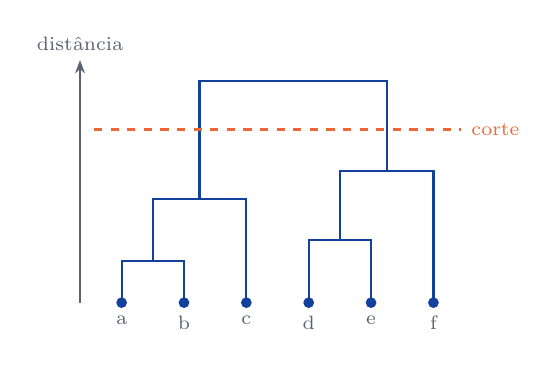
\begin{tikzpicture}[scale=0.88,font=\scriptsize]
        \foreach \x/\l in {0/a,0.9/b,1.8/c,2.7/d,3.6/e,4.5/f} {
          \fill[navy] (\x,0) circle (2.2pt); \node[below,text=muted] at (\x,-0.05) {\l};}
        \draw[navy,thick] (0,0) -- (0,0.6) -- (0.9,0.6) -- (0.9,0);
        \draw[navy,thick] (2.7,0) -- (2.7,0.9) -- (3.6,0.9) -- (3.6,0);
        \draw[navy,thick] (1.8,0) -- (1.8,1.5) -- (0.45,1.5) -- (0.45,0.6);
        \draw[navy,thick] (4.5,0) -- (4.5,1.9) -- (3.15,1.9) -- (3.15,0.9);
        \draw[navy,thick] (1.125,1.5) -- (1.125,3.2) -- (3.825,3.2) -- (3.825,1.9);
        \draw[-{Stealth},muted] (-0.6,0) -- (-0.6,3.5) node[above,text=muted] {distância};
        \draw[accent,dashed,thick] (-0.4,2.5) -- (4.9,2.5) node[right,text=accent] {corte};
      \end{tikzpicture}
    \end{plain}
    \column{0.54\textwidth}
    \begin{itemize}\normalsize\setlength{\itemsep}{4pt}
      \item Cada amostra começa sozinha; os \textbf{dois grupos mais próximos} se unem, até sobrar um
      \item Resultado: uma árvore, o \textbf{dendrograma}
      \item Cortamos a árvore no \textbf{mesmo $k=5$}
    \end{itemize}
    \vspace{2pt}
    \begin{card}{Ward = mesmo critério do k-means}
      Une o par que \textbf{menos aumenta a variância interna}: a comparação entre os métodos é justa.
    \end{card}
    \code{linkage(X, "ward")}\ \code{fcluster(Z, 5, "maxclust")}
  \end{columns}
\end{frame}

% ------------------------------------------------------------------ 10. Dendrograma
\begin{frame}{O dendrograma}
  \framesubtitle{\nbsec{3.4–3.5}}
  \vspace{0.0cm}
  \centering
  \begin{plain}[left=0.5mm,right=0.5mm,top=0.5mm,bottom=0.5mm,width=0.68\linewidth]
    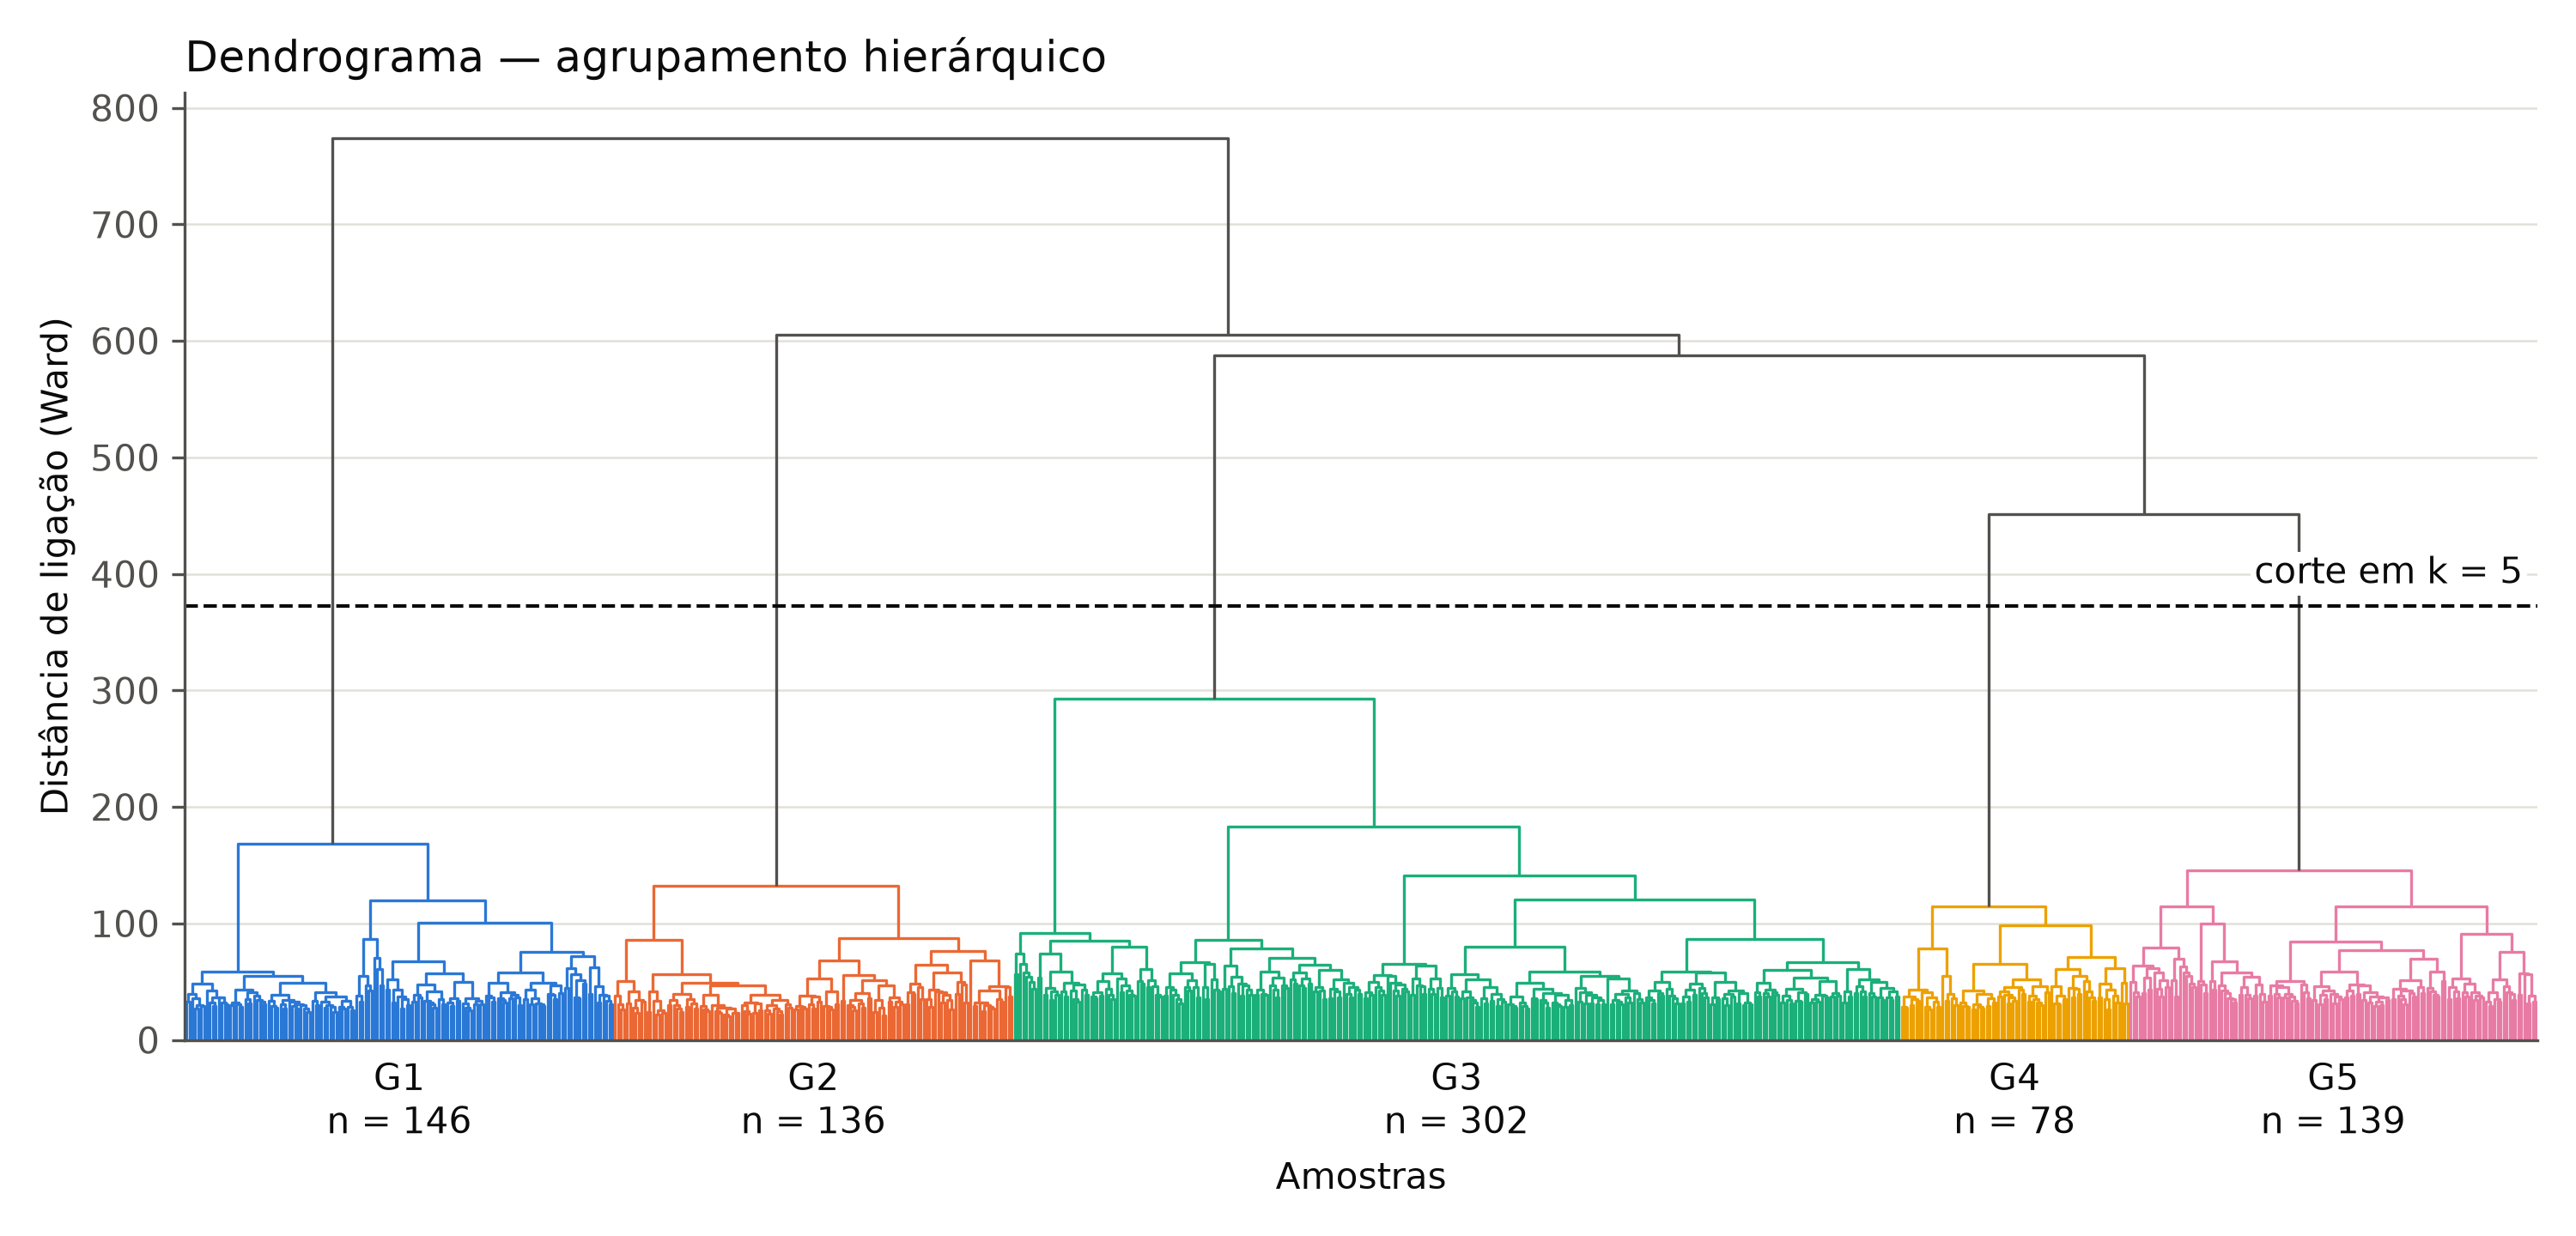
\includegraphics[width=\linewidth]{fig_dendrograma.png}
  \end{plain}
  \vspace{0.0cm}
  \begin{columns}[T,onlytextwidth]
    \column{0.32\textwidth}
    \begin{plain}[fontupper=\footnotesize]\centering
      \textbf{5 ramos bem definidos} abaixo do corte
    \end{plain}
    \column{0.32\textwidth}
    \begin{plain}[fontupper=\footnotesize]\centering
      Tamanhos \textbf{quase iguais} aos do k-means
    \end{plain}
    \column{0.32\textwidth}
    \begin{plain}[fontupper=\footnotesize]\centering
      G3 se divide e G4+G5 se unem \textbf{perto do corte}
    \end{plain}
  \end{columns}
\end{frame}

% ================================================================== PARTE 3
\setpart{Parte 3 · Julio Fuganti}

% ------------------------------------------------------------------ 11. Contingência
\newcommand{\hit}[1]{\cellcolor{okc!28}\textbf{#1}}
\newcommand{\miss}[1]{\cellcolor{errc!22}\textbf{\color{errc!80!black}#1}}
\newcommand{\z}{{\color{muted!60}0}}
\begin{frame}{Só agora: os rótulos}
  \framesubtitle{Tabelas de contingência: grupos encontrados × tipos reais — \nbsec{4.2–4.3}}
  \vspace{0.1cm}
  \begin{columns}[T,onlytextwidth]
    \column{0.48\textwidth}
    \begin{card}{k-means}
      \centering\footnotesize\setlength{\tabcolsep}{4pt}
      \resizebox{0.92\linewidth}{!}{\begin{tabular}{l|ccccc}
        & BRCA & COAD & KIRC & LUAD & PRAD\\\hline
        G1 & \hit{300} & \z & \miss{1} & \miss{2} & \z\\
        G2 & \z & \z & \hit{145} & \z & \z\\
        G3 & \z & \z & \z & \z & \hit{136}\\
        G4 & \z & \miss{1} & \z & \hit{139} & \z\\
        G5 & \z & \hit{77} & \z & \z & \z
      \end{tabular}}\par\vspace{5pt}
      \bignum{navy}{797 / 801}\ {\small no grupo certo}
    \end{card}
    \column{0.48\textwidth}
    \begin{card}{Hierárquico (Ward)}
      \centering\footnotesize\setlength{\tabcolsep}{4pt}
      \resizebox{0.92\linewidth}{!}{\begin{tabular}{l|ccccc}
        & BRCA & COAD & KIRC & LUAD & PRAD\\\hline
        G1 & \z & \z & \hit{146} & \z & \z\\
        G2 & \z & \z & \z & \z & \hit{136}\\
        G3 & \hit{300} & \z & \z & \miss{2} & \z\\
        G4 & \z & \hit{78} & \z & \z & \z\\
        G5 & \z & \z & \z & \hit{139} & \z
      \end{tabular}}\par\vspace{5pt}
      \bignum{navy}{799 / 801}\ {\small no grupo certo}
    \end{card}
  \end{columns}
  \vspace{0.05cm}
  \centering{\small Cada grupo tem \textbf{$\geq$ 99\%} de um único tipo. A numeração dos grupos é arbitrária.\par}
\end{frame}

% ------------------------------------------------------------------ 12. PCA
\begin{frame}{Os grupos na PCA}
  \framesubtitle{\nbsec{5.2–5.3}}
  \vspace{0.0cm}
  \centering
  \begin{plain}[left=0.5mm,right=0.5mm,top=0.5mm,bottom=0.5mm,width=0.72\linewidth]
    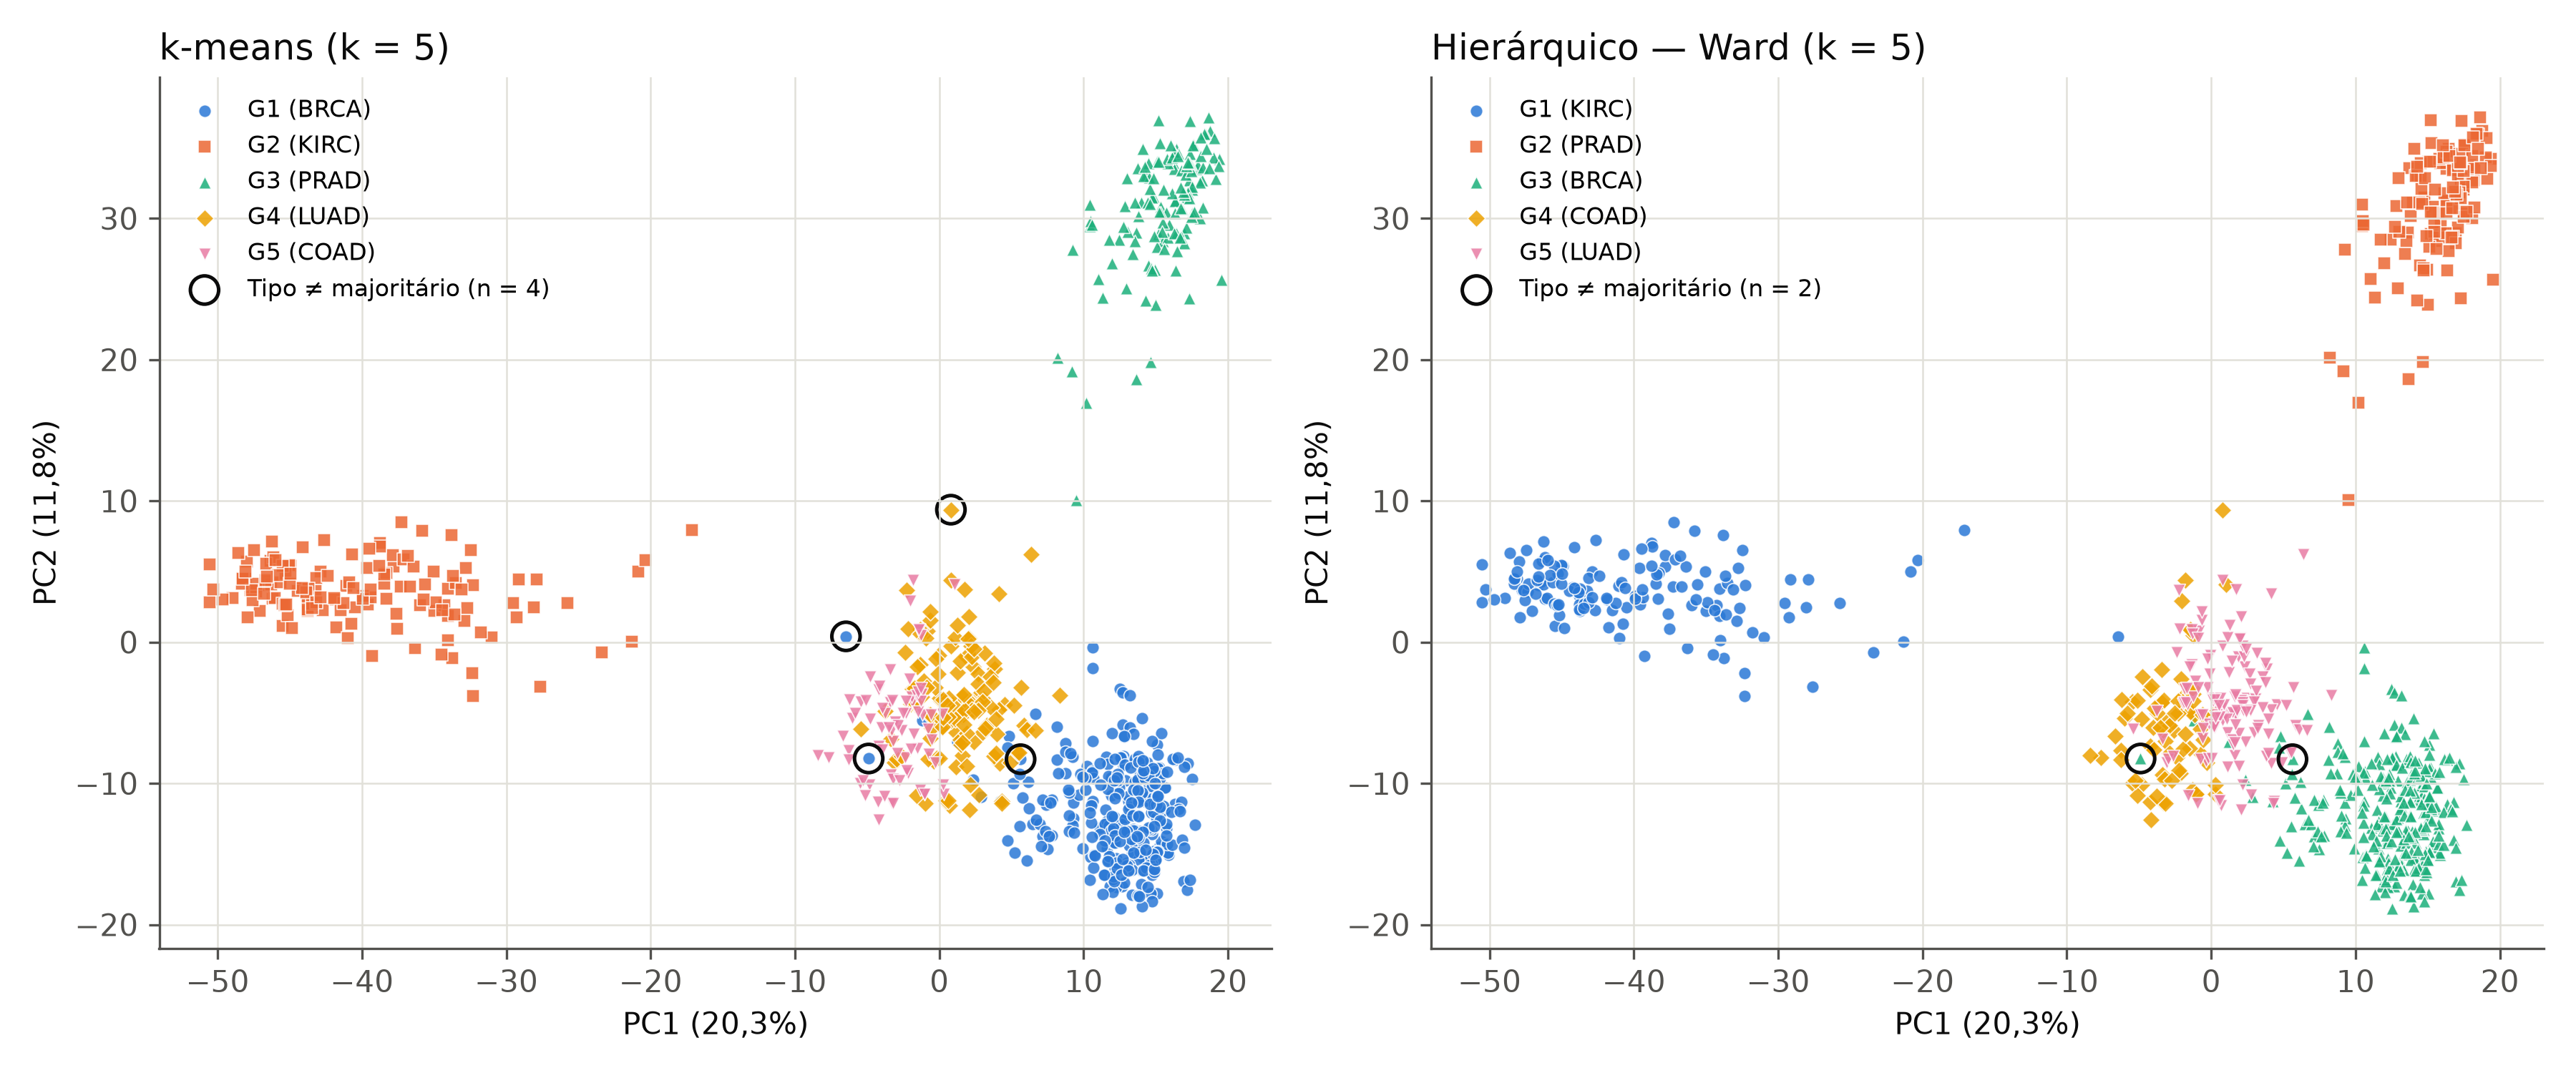
\includegraphics[width=\linewidth]{fig_pca_grupos.png}
  \end{plain}
  \vspace{0.0cm}
  \begin{columns}[T,onlytextwidth]
    \column{0.32\textwidth}
    \begin{plain}[fontupper=\footnotesize]\centering
      O plano mostra só \textbf{32\%} da variância
    \end{plain}
    \column{0.32\textwidth}
    \begin{plain}[fontupper=\footnotesize]\centering
      LUAD e COAD se sobrepõem aqui, mas são separados nos \textbf{2.000 genes}
    \end{plain}
    \column{0.32\textwidth}
    \begin{plain}[fontupper=\footnotesize]\centering
      Os erros (círculos) ficam nas \textbf{fronteiras}
    \end{plain}
  \end{columns}
\end{frame}

% ------------------------------------------------------------------ 13. Diferente não é errado
\begin{frame}{Diferente não é errado}
  \framesubtitle{O mesmo dendrograma, cortado em outras alturas}
  \vspace{0.1cm}
  \begin{columns}[T,onlytextwidth]
    \column{0.50\textwidth}
    \begin{plain}
      \centering
      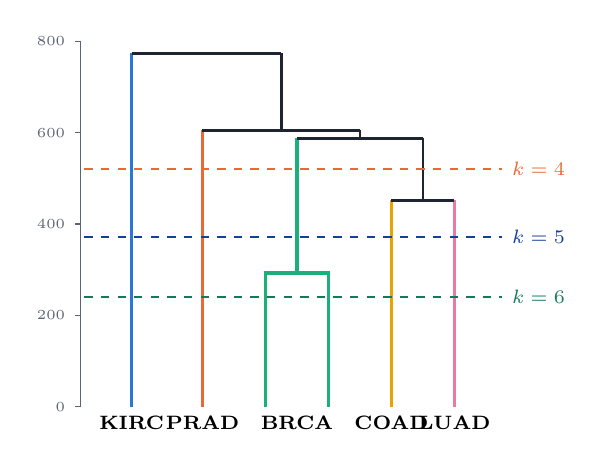
\begin{tikzpicture}[yscale=0.58,xscale=1.0,font=\scriptsize]
        \draw[muted] (-0.35,0) -- (-0.35,8);
        \foreach \v/\t in {0/0,2/200,4/400,6/600,8/800} {\draw[muted] (-0.42,\v) -- (-0.35,\v);
          \node[left,text=muted,font=\tiny] at (-0.42,\v) {\t};}
        \draw[c1,line width=1.3pt] (0.3,0) -- (0.3,7.74);
        \draw[c2,line width=1.3pt] (1.2,0) -- (1.2,6.05);
        \draw[c3,line width=1.3pt] (2.0,0) -- (2.0,2.93) -- (2.8,2.93) -- (2.8,0);
        \draw[c3,line width=1.3pt] (2.4,2.93) -- (2.4,5.88);
        \draw[c4,line width=1.3pt] (3.6,0) -- (3.6,4.52);
        \draw[c5,line width=1.3pt] (4.4,0) -- (4.4,4.52);
        \draw[ink,line width=1pt] (3.6,4.52) -- (4.4,4.52); \draw[ink,line width=1pt] (4.0,4.52) -- (4.0,5.88);
        \draw[ink,line width=1pt] (2.4,5.88) -- (4.0,5.88); \draw[ink,line width=1pt] (3.2,5.88) -- (3.2,6.05);
        \draw[ink,line width=1pt] (1.2,6.05) -- (3.2,6.05); \draw[ink,line width=1pt] (2.2,6.05) -- (2.2,7.74);
        \draw[ink,line width=1pt] (0.3,7.74) -- (2.2,7.74);
        \draw[accent,dashed,thick] (-0.3,5.2) -- (5.0,5.2) node[right] {$k=4$};
        \draw[navy,dashed,thick] (-0.3,3.72) -- (5.0,3.72) node[right] {$k=5$};
        \draw[okc!70!black,dashed,thick] (-0.3,2.4) -- (5.0,2.4) node[right] {$k=6$};
        \foreach \x/\l in {0.3/KIRC,1.2/PRAD,2.4/BRCA,3.6/COAD,4.4/LUAD}
          \node[below,font=\scriptsize\bfseries] at (\x,0) {\l};
      \end{tikzpicture}\par
      {\tiny\color{muted}Esquema do topo da árvore (alturas aproximadas).}
    \end{plain}
    \column{0.46\textwidth}
    \begin{itemize}\normalsize\setlength{\itemsep}{4pt}
      \item \textbf{$k=4$:} COAD + LUAD juntos
      \item \textbf{$k=5$:} os 5 tipos de tumor
      \item \textbf{$k=6$:} BRCA dividido em dois
    \end{itemize}
    \vspace{0.15cm}
    \begin{card}{Por quê?}
      O método minimiza a \textbf{variância interna}, não procura “tipos de tumor”.\par\vspace{3pt}
      O resultado depende de \textbf{$k$, genes, padronização e ligação}. Cada corte mostra uma estrutura real, em outra escala.
    \end{card}
  \end{columns}
\end{frame}

% ------------------------------------------------------------------ 14. Respostas
\begin{frame}{Respostas às perguntas}
  \vspace{0.25cm}
  \begin{card}[fontupper=\normalsize]{O cotovelo apontou $k = 5$?}
    \textbf{Sim}, mas por pouco: o cotovelo é suave e $k=4$ ficou logo atrás.
  \end{card}
  \begin{card}[fontupper=\normalsize]{Algum tipo foi dividido ou misturado?}
    \textbf{Não}: cada grupo tem $\geq$ 99\% de um tipo. Só 4 (k-means) e 2 (Ward) amostras fora do lugar.
  \end{card}
  \begin{card}[fontupper=\normalsize]{Por que uma divisão diferente pode estar certa?}
    O método otimiza \textbf{geometria}, não rótulos: outro $k$ revela outra estrutura real dos dados.
  \end{card}
\end{frame}

% ------------------------------------------------------------------ 15. Conclusões
\begin{frame}{Conclusões}
  \vspace{0.3cm}
  \begin{columns}[T,onlytextwidth]
    \column{0.32\textwidth}
    \begin{card}[height=2.9cm,fontupper=\normalsize]{O sinal é forte}
      Sem rótulos, os 5 tipos foram redescobertos com \textbf{> 99\%} de acerto.
    \end{card}
    \column{0.32\textwidth}
    \begin{card}[height=2.9cm,fontupper=\normalsize]{Métodos concordam}
      k-means e Ward, com o mesmo critério, chegaram a grupos \textbf{quase idênticos}.
    \end{card}
    \column{0.32\textwidth}
    \begin{card}[height=2.9cm,fontupper=\normalsize,colbacktitle=accent]{$k$ é a escolha crítica}
      A estrutura existe em \textbf{várias escalas}; o $k$ decide qual delas vemos.
    \end{card}
  \end{columns}
  \vspace{0.5cm}
  \centering
  {\titlefont\fontsize{26}{28}\selectfont\color{titlecol}OBRIGADO!\par}
\end{frame}

\end{document}
